\chapter{Figures and Astronomical Notation}
\label{ch:astronomy}

\section{Figures}
\label{sec:figures}

Place your images in \file{content/figures/}. Because \file{thesis.tex} sets \cmd{graphicspath} to that folder, \cmd{includegraphics} only needs the file name. Figure~\ref{fig:bibliography-process} in Chapter~\ref{ch:bibliographies} was included with:
\begin{lstlisting}[language=TeX]
\begin{figure}[htbp]
    \centering
    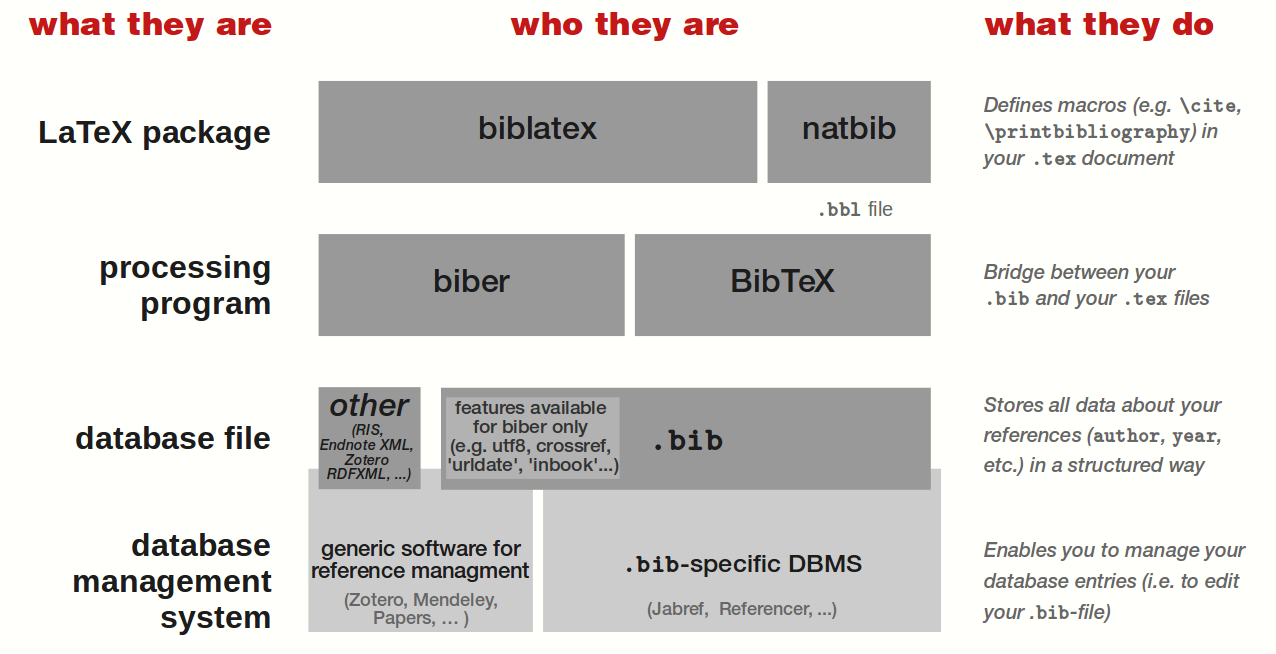
\includegraphics[width=0.8\textwidth]{citations_overview.png}
    \caption{Bibliography Process Overview in \LaTeX}
    \label{fig:bibliography-process}
\end{figure}
\end{lstlisting}
Always give a figure a \cmd{caption} (this is what appears in the List of Figures) and a \cmd{label}, and refer to it in the text with \cmd{ref}. Figures with several panels can use the \texttt{subfigure} environment from the \texttt{subcaption} package, which the class loads. Vector formats (PDF) stay sharp at any zoom level; use PNG or JPEG only for photographs and images.

\section{Astronomical Notation}
\label{sec:notation}

The class provides the notation macros of the AASTeX journal class, so that text using them can be copied from a paper written with AASTeX. They work in normal text; Table~\ref{tab:notation} lists them.

\begin{table}[htbp]
    \centering
    \caption[Astronomical notation macros provided by the class]{Astronomical notation macros provided by the class.}
    \label{tab:notation}
    \begin{tabularx}{\linewidth}{@{}l l >{\raggedright\arraybackslash}X@{}}
        \toprule
        Command & Output & Meaning \\
        \midrule
        \cmd{arcdeg}, \cmd{degr} & 5\arcdeg & degrees \\
        \cmd{arcmin} & 5\arcmin & arcminutes \\
        \cmd{arcsec} & 5\arcsec & arcseconds \\
        \cmd{fd}, \cmd{fh}, \cmd{fm}, \cmd{fs} & 2\fd5, 12\fh5, 30\fm5, 45\fs5 & fractional day, hour, minute, second \\
        \cmd{fdg}, \cmd{farcm}, \cmd{farcs} & 3\fdg2, 4\farcm5, 0\farcs75 & fractional degree, arcminute, arcsecond \\
        \cmd{fp} & 1\fp5 & fractional parallax \\
        \cmd{micron} & 2.2~\micron & micrometres \\
        \cmd{ion}\texttt{\{Fe\}\{2\}} & \ion{Fe}{2} & ionization state \\
        \cmd{la}, \cmd{ga} & $z \la 2$, $z \ga 2$ & less / greater than about \\
        \cmd{ubvr}, \cmd{ub}, \cmd{bv}, \cmd{vr}, \cmd{ur} & \ubvr, \ub, \bv, \vr, \ur & photometric bands and colours \\
        \cmd{case}\texttt{\{1\}\{3\}}, \cmd{onehalf} & \case{1}{3}, \onehalf & fractions in running text \\
        \bottomrule
    \end{tabularx}
\end{table}

Note that \cmd{la} and \cmd{ga} must be used in math mode, as in \verb|$z \la 2$|.

For the fractional units, put the macro where the decimal point goes: \verb|12\fh5| gives 12\fh5.

\section{Aligning Numbers in Tables}
\label{sec:phantoms}

The class also provides the AASTeX ``phantom'' commands, which insert invisible space the width of a character so that columns of numbers line up:
\begin{center}
    \begin{tabular}{@{}l l@{}}
        \toprule
        Command & Inserts the width of \\
        \midrule
        \cmd{phn} & a digit \\
        \cmd{phd} & a decimal point \\
        \cmd{phs} & a minus sign \\
        \cmd{phm}\texttt{\{text\}} & any text \\
        \bottomrule
    \end{tabular}
\end{center}

\section{Symbols}
\label{sec:symbols}

Solar units are written in math mode with \verb|\odot|, for example \verb|$M_\odot$| gives $M_\odot$. The \texttt{wasysym} package, loaded by the class, provides further astronomical symbols for use in text, such as \cmd{sun} (\sun), \cmd{mercury} (\mercury), \cmd{venus} (\venus), \cmd{earth} (\earth), \cmd{mars} (\mars), \cmd{jupiter} (\jupiter), and \cmd{saturn} (\saturn). The full list is in the \texttt{wasysym} documentation.
